\documentclass[12pt, titlepage]{article}

\usepackage{graphicx}
\usepackage{booktabs}
\usepackage{tabularx}
\usepackage{float}
\usepackage{hyperref}
\hypersetup{
    colorlinks,
    citecolor=black,
    filecolor=black,
    linkcolor=red,
    urlcolor=blue
}
\usepackage[round]{natbib}

\title{SE 3XA3: Software Requirements Specification\\Node Messenger}

\author{Team \#24, Node Messenger
		\\ Tasin Ahmed - ahmedm31
		\\ Shardool Patel - pates25
		\\ Omar Elemary - elemaryo
}

\date{\today}

\begin{document}
    \maketitle

    \pagenumbering{roman}
    \tableofcontents
    \listoftables
    \listoffigures

    \begin{table}[bp]
    \caption{\bf Revision History}
    \begin{tabularx}{\textwidth}{p{3cm}p{2cm}X}
    \toprule {\bf Date} & {\bf Version} & {\bf Notes}\\
    \midrule
    Date 1 & 1.0 & Notes\\
    Date 2 & 1.1 & Notes\\
    \bottomrule
    \end{tabularx}
    \end{table}

    \newpage

    \pagenumbering{arabic}

    This document describes the requirements for ....  The template for the Software
    Requirements Specification (SRS) is a subset of the Volere
    template~\citep{RobertsonAndRobertson2012}.  If you make further modifications
    to the template, you should explicity state what modifications were made.

    \section{Project Drivers}

    	\subsection{The Purpose of the Project}
<<<<<<< HEAD

    	\subsection{The Stakeholders}

    		\subsubsection{The Client}

    		\subsubsection{The Customers}

    		\subsubsection{Other Stakeholders}

    	\subsection{Mandated Constraints}

    	\subsection{Naming Conventions and Terminology}

    	\subsection{Relevant Facts and Assumptions}

    	User characteristics should go under assumptions.
=======
        As the world becomes increasingly more connected through the internet, many common internet users are looking for an easy way to communicate with each other or reach out to distant loved ones. The market for messengers has become saturated with products that put the goal of earning maximum revenue over the needs of the consumer. Our team’s focus is to gauge consumer interest by implementing a free and accessible web application messenger that allows them to personalize their experience and chat with other users in a simple, clean and non-intrusive way. Node messenger will become a haven for users searching for a consumer-friendly product with great functionality and cross-platform support.
    	\subsection{The Stakeholders}

    		\subsubsection{The Client}
            The client for Node Messenger would be the same as the end user since Node Messenger is a general purpose app designed to serve anyone with access to internet.
    		\subsubsection{The Customers}
    		Node messenger will serve as a general purpose chat application that also supports group chats. The customers for Node messenger will be - the people who want to connect with friends and family, various discussion groups and collaborative teams.


    		\subsubsection{Other Stakeholders}
    		 Other stakeholders included the development team and future developers who might want to build upon this open source project.

    	\subsection{Mandated Constraints}
    Not Applicable
    	\subsection{Naming Conventions and Terminology}
Not Applicable
    	\subsection{Relevant Facts and Assumptions}

    	-Users will comply with policies of use and will not try to intentionally ruin the experience for other users\\
    	-One server can handle all the users
>>>>>>> 6d3c2f54d306e701e80898be9eb6045a5256a15b
	
	\newpage
    \section{Functional Requirements}

    	\subsection{The Scope of the Work and the Product}

    		\subsubsection{The Context of the Work}
<<<<<<< HEAD

    		\subsubsection{Work Partitioning}

    		\subsubsection{Individual Product Use Cases}

    	\subsection{Functional Requirements}
	
=======
    		\subsubsection{Work Partitioning}
    		\subsubsection{Individual Product Use Cases}
    		 
            \begin{figure}[H]
                \centering
                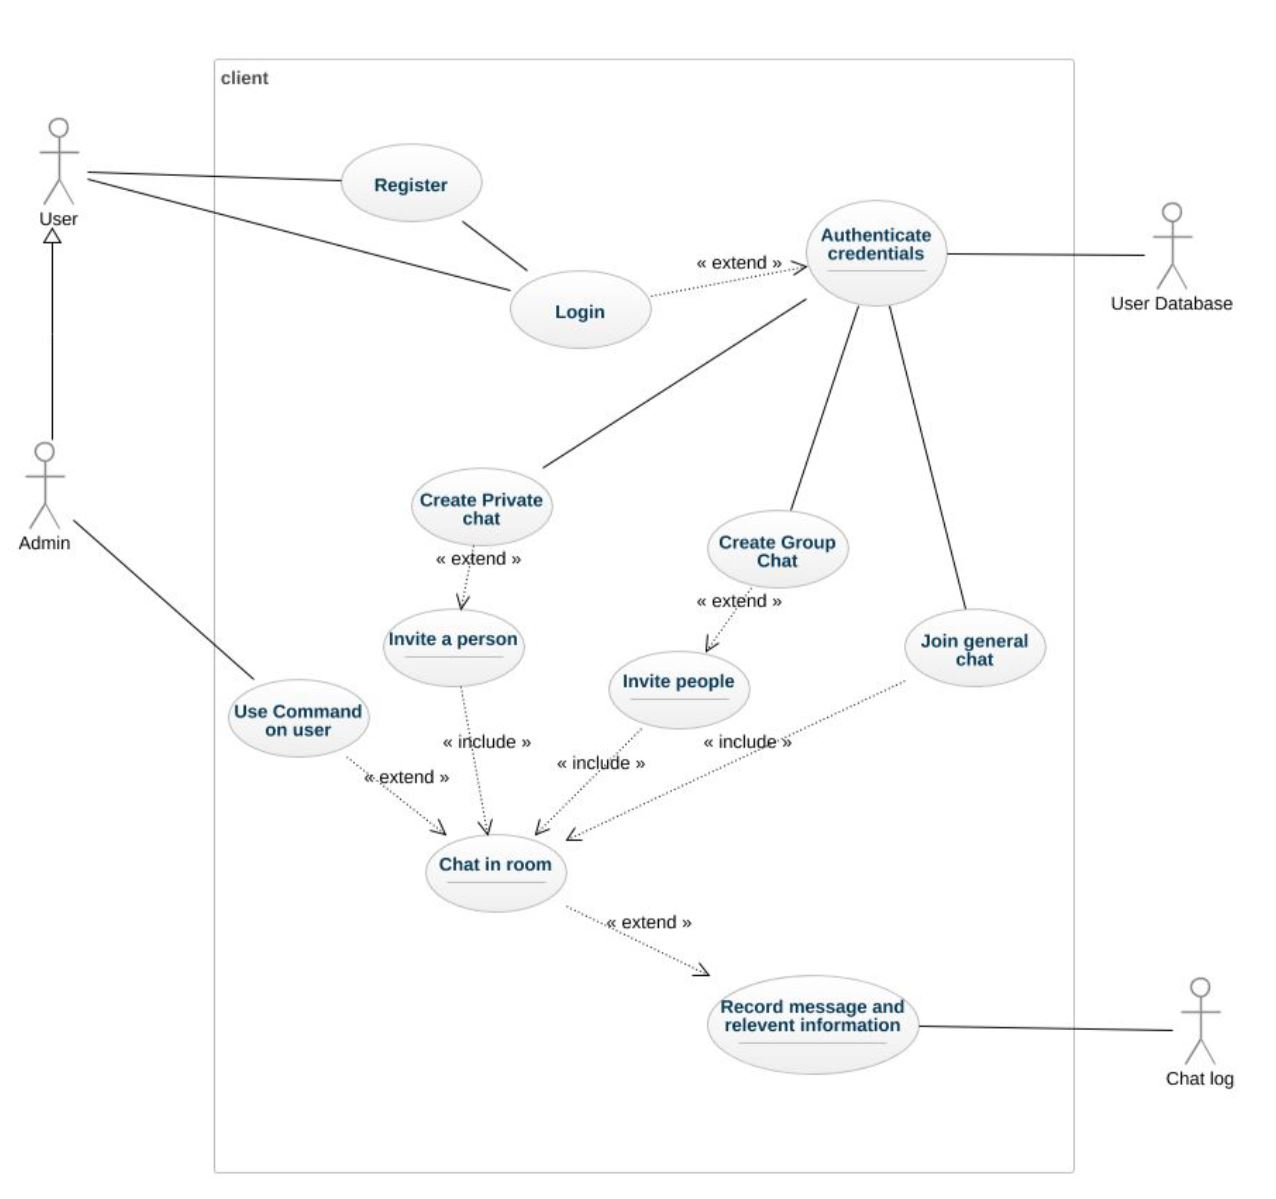
\includegraphics[scale=0.6]{diagram.jpg}
                \caption{Example Use Case}
                \label{fig:my_label}
            \end{figure}
           
           

    		
    		

    	\subsection{Functional Requirements}
	    \begin{enumerate}
		    \item The software shall be free to access by all users through the web app or cross platform app.
		    \item The software shall allow user to log-in to web app messenger using user name or email address and password.
		    \item The software shall allow user to remember their log-in information on the web app for easier and faster access.
		    \item The software shall allow users to log-out and log-in to the system at will.
		    \item The software shall allow user to create an account with Node Messenger by providing name, user name, email address, password and profile picture.
		    \item The software shall validate new accounts with the use of randomly generated verification codes sent to the user's email address.
		    \item The software shall allow communication through one-on-one messaging between other Node Messenger users.
		    \item The software shall allow the user to discover other users by attached email or phone numbers.
		    \item The software shall allow the user to create group
		    conversation of 128 other Node Messenger users independent of friendship status.
		    \item The software shall allow the user to modify group conversation settings by changing its name and picture, add and remove members or leave group based on administrative status.
		    \item The software shall give the user control over individual conversations with the ability to delete chat and mute or block other user.
		    \item The software shall display the online and offline status of other Node Messenger users using green circle for online and grey circle for offline status.
		    \item The software shall allow the user to access other user's profile information via the info tab.
		    \item The software shall support persistent message storing of multiple chats with paginated message history.
		    \item The software shall distinguish between user sent and received messages using a different color scheme for each situation.
		    \item The software shall display an indicator for the number of unread messages besides chat menu and beside the browser tab name.
		    \item The software shall allow user to transmit documents, photos and videos of many file formats to other users.
		    \item The software shall send server-generated notification alerts and message sounds to the user whenever a message is received.
		    \item The software shall display message status notification indicating message delivery to server, received and read notifications and typing notifications.
		    \item The software shall allow the user to mute notification alerts and message sounds from Node Messenger.
		    \item The software shall allow user to modify their profile by changing their profile picture, name and password.
		    \item The software shall support font modifications such as bolding and italics.
		    \item The software shall support different languages and emojis.
		\end{enumerate}
>>>>>>> 6d3c2f54d306e701e80898be9eb6045a5256a15b
	\newpage
    \section{Non-functional Requirements}

    	\subsection{Look and Feel Requirements}
    	The users will be we greeted by a welcome page with logo of our product, information, and contacts. There will be two buttons named 'Register' and 'Login' which they can use to begin using the Node Messenger. The Node Messenger will be in a different tab, and can be accessed with the click of a button.The welcome page should be visibly appealing and be structured well for the ease of use. The messenger itself should have a simple yet unique design, as to not make it cluttered and difficult to use.

    	\subsection{Usability and Humanity Requirements}
		Node Messenger can be used by anyone with the need to communicate with others over the Internet. The user should be able to access the website through our URL, be able to use a keyboard and mouse to navigate around our website. Previous knowledge of other messaging apps can be helpful. The user should be able to access the website through our URL, be able to use a keyboard and mouse to navigate around our website. Previous knowledge of other messaging apps can be helpful. Node Messenger can be accessed on any browser, and mobile as we plan to make it responsive.
    	\subsection{Performance Requirements}
		Node Messenger should be quick to respond to user instructions, while transferring and receiving messages as quickly as possible. It should keep the user's personal data safe, and keep the machine's memory usage to a minimum. Node Messenger should be available to user anywhere on Earth with the access to Internet. It should be able to provide service to many users at the same time. It can be used on any browser without the need to be downloaded on the machine. Our HTML code with account for scalability of the messenger. Node Messenger shall be usable as long as HTML, CSS, and Javascript is supported by the browser.
    	\subsection{Operational and Environmental Requirements}
		Node Messenger can be used on any browser that supports the latest versions of HTML, CSS, and Javascript. Before Node Messenger can be used, it must be able to run on a local URL, and be responsive. We plan to update Node Messenger as frequently as possible to keep the features up-to-date.
    	\subsection{Maintainability and Support Requirements}
		We will check for errors before release in order to keep maintenance to a minimum. Wee will also ensure Node Messenger can run on the majority of the browsers. Node Messenger should be available to anyone with the URL, and access to Internet.
    	\subsection{Security Requirements}
		Node Messenger can be accessed by anyone, given their machine meets the minimum requirements. it should not let users with invalid credentials login. Node Messenger should preserve the personal data of the users.
    	\subsection{Cultural Requirements}
		Node Messenger should be respectful of all users of different cultures and backgrounds. It will be available in English, be hosted on North American servers. It will be available worldwide. 
	    \subsection{Legal Requirements}
		Node Messenger shall not disobey any laws.
    	\subsection{Health and Safety Requirements}
		We will make sure the colors used do not put too much pressure on the eyes. 
	
	\newpage
    \section{Project Issues}

    	\subsection{Open Issues}
    	Not Applicable.

    	\subsection{Off-the-Shelf Solutions}
<<<<<<< HEAD
    	Not Applicable.
=======
    	\begin{enumerate}
    	    \item Tinode Messenger
    	    \item Facebook Messenger
    	    \item Discord
    	\end{enumerate}
>>>>>>> 6d3c2f54d306e701e80898be9eb6045a5256a15b

    	\subsection{New Problems}
    	Node Messenger will occupy just one of the many web addresses being hosted. It should not create any problems, unless the website cannot hold a large amount of people at a time. The product will not have any effect on the installed systems, as nothing is required to be downloaded to be used. Node Messenger might cause problems for the users if used for a prolonged period of time, such as hand pain, or eye soreness. 

    	\subsection{Tasks}
    	\begin{center}
    		\begin{tabular}{|c|c|c|}
    		\hline 
    		Task & Completer's Role & Timeline \\ 
    		\hline 
    		Model Implementation & Software Engineer & Oct 10th \\ 
    		\hline 
    		Model Revision & Client & Oct 14th \\ 
    		\hline 
    		HTML and CSS implementation & Software Engineers & Oct 25th \\ 
    		\hline 
    		Javascript backend & Software Engineers &  Nov 1st\\ 
    		\hline 
    		Revision & Client & Nov 3rd \\ 
    		\hline 
    		Host Node Messenger& Software Engineers & Nov 24th \\ 
    		\hline 
    		Maintenance & Software Engineers & Yearly \\ 
    		\hline 
    	\end{tabular} 
    	\end{center}
		Task 1: Create a model of the Node Messenger website to visualize how everything will be positioned. This will help to understand how everything in our website will interact with each other. Task 2: Create the front-end of the website using HTML and CSS. Ensure the website is clean and visually appealing. Task 3: Create the back-end of the website using Javascript. Ensure all components of the messenger is fully functioning and creates the desired output. Task 4: Host the messaging app on a free web hosting site.
<<<<<<< HEAD
		
    	\subsection{Migration to the New Product}

    	\subsection{Risks}

    	\subsection{Costs}

    	\subsection{User Documentation and Training}

    	\subsection{Waiting Room}

    	\subsection{Ideas for Solutions}
=======

    	\subsection{Migration to the New Product}
    	Not Applicable.

    	\subsection{Risks}
    	Not Applicable.

    	\subsection{Costs}
    	None as long as our web-hosting is free.

    	\subsection{User Documentation and Training}
    	Not Applicable.

    	\subsection{Waiting Room}
    	Not Applicable.

    	\subsection{Ideas for Solutions}
    	Proper coding indentation, structure and documentation.
>>>>>>> 6d3c2f54d306e701e80898be9eb6045a5256a15b

	\newpage
    \bibliographystyle{plainnat}

    \bibliography{SRS}


    \section{Appendix}

    This section has been added to the Volere template.  This is where you can place
    additional information.

    \subsection{Symbolic Parameters}

    The definition of the requirements will likely call for SYMBOLIC\_CONSTANTS.
    Their values are defined in this section for easy maintenance.


\end{document}